\section{Public-data mechanism checks}
\label{app:public-checks}

This appendix uses public data to examine outcomes around synchronized delivered policy easing. The event is intentionally later than the yield-curve state: inversions can encode expected easing, whereas policy-rate cuts record policymakers' actions. The exercise tests selected mechanism implications but, because it observes policy delivery rather than the predictive state, it does not validate the inversion classifier.

\subsection{Event construction}

The sample is January 1988 through December 2025. Let $r^{pol}_{i,t}$ be country $i$'s BIS end-of-period policy rate and define
\begin{equation}
K_{i,t}=\1\{\Delta r^{pol}_{i,t}\leq-0.10\},
\qquad
B_t=\sum_iK_{i,t},
\label{eq:public-cuts}
\end{equation}
where rates and the 10-basis-point cutoff are in percentage points. Let $D_t=1$ when $B_t\geq3$ and at least six country rates are observed. The onset indicator is
\begin{equation}
O_t=D_t\prod_{\ell=1}^{3}(1-D_{t-\ell}).
\label{eq:public-onset}
\end{equation}
Thus an onset requires at least three cutting countries after three months without another synchronized-cut month. The rule produces fifteen onsets. These fifteen public easing onsets are not the paper's fifteen inversion episodes; the identical counts are coincidental.

The public currency outcome is a spot-only proxy. BIS exchange rates are signed so that a positive return is foreign-currency appreciation against the dollar. At $t-1$, currencies are ranked by their policy-rate differentials against the United States; the proxy is long the three highest-ranked and short the three lowest-ranked. The rank is predetermined, but $O_t$ is observed during month $t$, so month-$t$ returns are contemporaneous event associations rather than feasible predictions made before easing.

Additional outcomes are CFTC non-commercial net positions scaled by open interest, the New York Fed ACM 10-year expected-rate and term-premium components \citep{adrian2013}, the OECD G7 composite leading indicator, NFCI, and VIX. CFTC coverage is limited to seven directly matchable contracts and uses a documented Deutsche-mark/euro convention. ACM is a U.S. diagnostic, not a decomposition of the nine foreign slopes. The macro and financial-condition series are current vintage.

\subsection{Event estimands and inference}

The code uses two estimands. For a level outcome $Y$, the horizon-$h$ event response is
\begin{equation}
\widehat\theta_h^{\mathrm{change}}
=\frac{1}{n_h}\sum_{j\in\mathcal J_h}
\left(Y_{\tau_j+h}-Y_{\tau_j-1}\right).
\label{eq:public-level-estimand}
\end{equation}
For a monthly return flow $R$, it is
\begin{equation}
\widehat\theta_h^{\mathrm{return}}
=\frac{1}{n_h}\sum_{j\in\mathcal J_h}
\sum_{\ell=0}^{h}R_{\tau_j+\ell},
\label{eq:public-return-estimand}
\end{equation}
where $\tau_j$ indexes valid onset dates. Ninety-percent intervals resample onset episodes; leave-one-onset ranges diagnose influence. The reference distribution enumerates circular shifts of the complete onset sequence, retains shifts with the observed number of valid event outcomes, includes the observed assignment, and doubles the smaller inclusive-tail rank. With irregular missingness, the retained shifts need not form a transformation group; the resulting values are conditional finite-rotation references, not exact causal randomization tests.

Six declared primary outcomes receive Holm adjustment: the shadow-carry spot return over months 0--1; the CFTC positioning change through month 3; ACM expected-rate and term-premium changes through month 3; the CLI change through month 6; and the NFCI change through month 3. The declaration is recorded in the analysis configuration and run manifest, but not in an immutable pre-analysis registration. VIX and other horizons are descriptive.

\begin{table}[!htbp]
\centering
\caption{Outcomes around synchronized delivered-easing onsets}
\label{tab:public_mechanism_checks}
\small
\begin{tabular}{>{\raggedright\arraybackslash}p{4.6cm}rrrrr}
\toprule
Outcome & Estimate & 90\% CI & RI $p$ & Holm $p$ & Rotations \\
\midrule
Policy-ranked shadow carry spot return, months 0--1 & -1.10 & [-3.55, 1.18] & 0.195 & 0.975 & 441 \\
Carry-aligned CFTC non-commercial net share, change through month 3 & -4.39 & [-13.53, 5.40] & 0.741 & 1.000 & 81 \\
ACM 10-year expected-rate component, change through month 3 & -0.13 & [-0.31, 0.07] & 0.202 & 0.975 & 396 \\
ACM 10-year term premium, change through month 3 & -0.03 & [-0.19, 0.14] & 0.980 & 1.000 & 396 \\
OECD G7 CLI, change through month 6 & -0.34 & [-0.72, 0.00] & 0.159 & 0.952 & 353 \\
Chicago Fed NFCI, change through month 3 & 0.03 & [-0.08, 0.15] & 0.520 & 1.000 & 396 \\
VIX, change through month 1 & 1.89 & [-2.30, 5.81] & 0.400 & -- & 20 \\
\bottomrule
\end{tabular}
\begin{minipage}{0.96\linewidth}\footnotesize Notes: Events are synchronized delivered-easing onsets constructed from public BIS policy rates. They are a downstream policy-rate state, distinct from the paper's predictive IYC state. RI $p$-values enumerate every circular rotation, condition on the observed number of valid episode outcomes, include the observed assignment, and double the smaller inclusive tail rank. Rotations reports the resulting finite reference count. The CFTC reference is small because missing contract coverage makes most rotations change the valid event count; its RI result is correspondingly coarse. With irregular missingness, the same-count rotations need not form a transformation group, so these are conditional finite-rotation references rather than exact causal randomization tests. Intervals resample onset episodes. Holm $p$-values adjust the six prespecified primary outcomes. Currency returns and CFTC positioning are percentage points, with CFTC positions measured as a share of open interest; ACM components are percentage points; CLI, NFCI, and VIX are index points.\end{minipage}
\end{table}


The signs mostly fit a broad stress-and-easing chronology: the shadow carry proxy depreciates, carry-aligned positions decline, the expected-rate component falls, and the leading indicator weakens. Estimates are imprecise, and no primary outcome survives the Holm adjustment. The U.S. term-premium estimate is nearly flat at three months. These results are directional mechanism evidence around policy delivery, not evidence that the inversion state predicts them.

\begin{figure}[H]
  \centering
  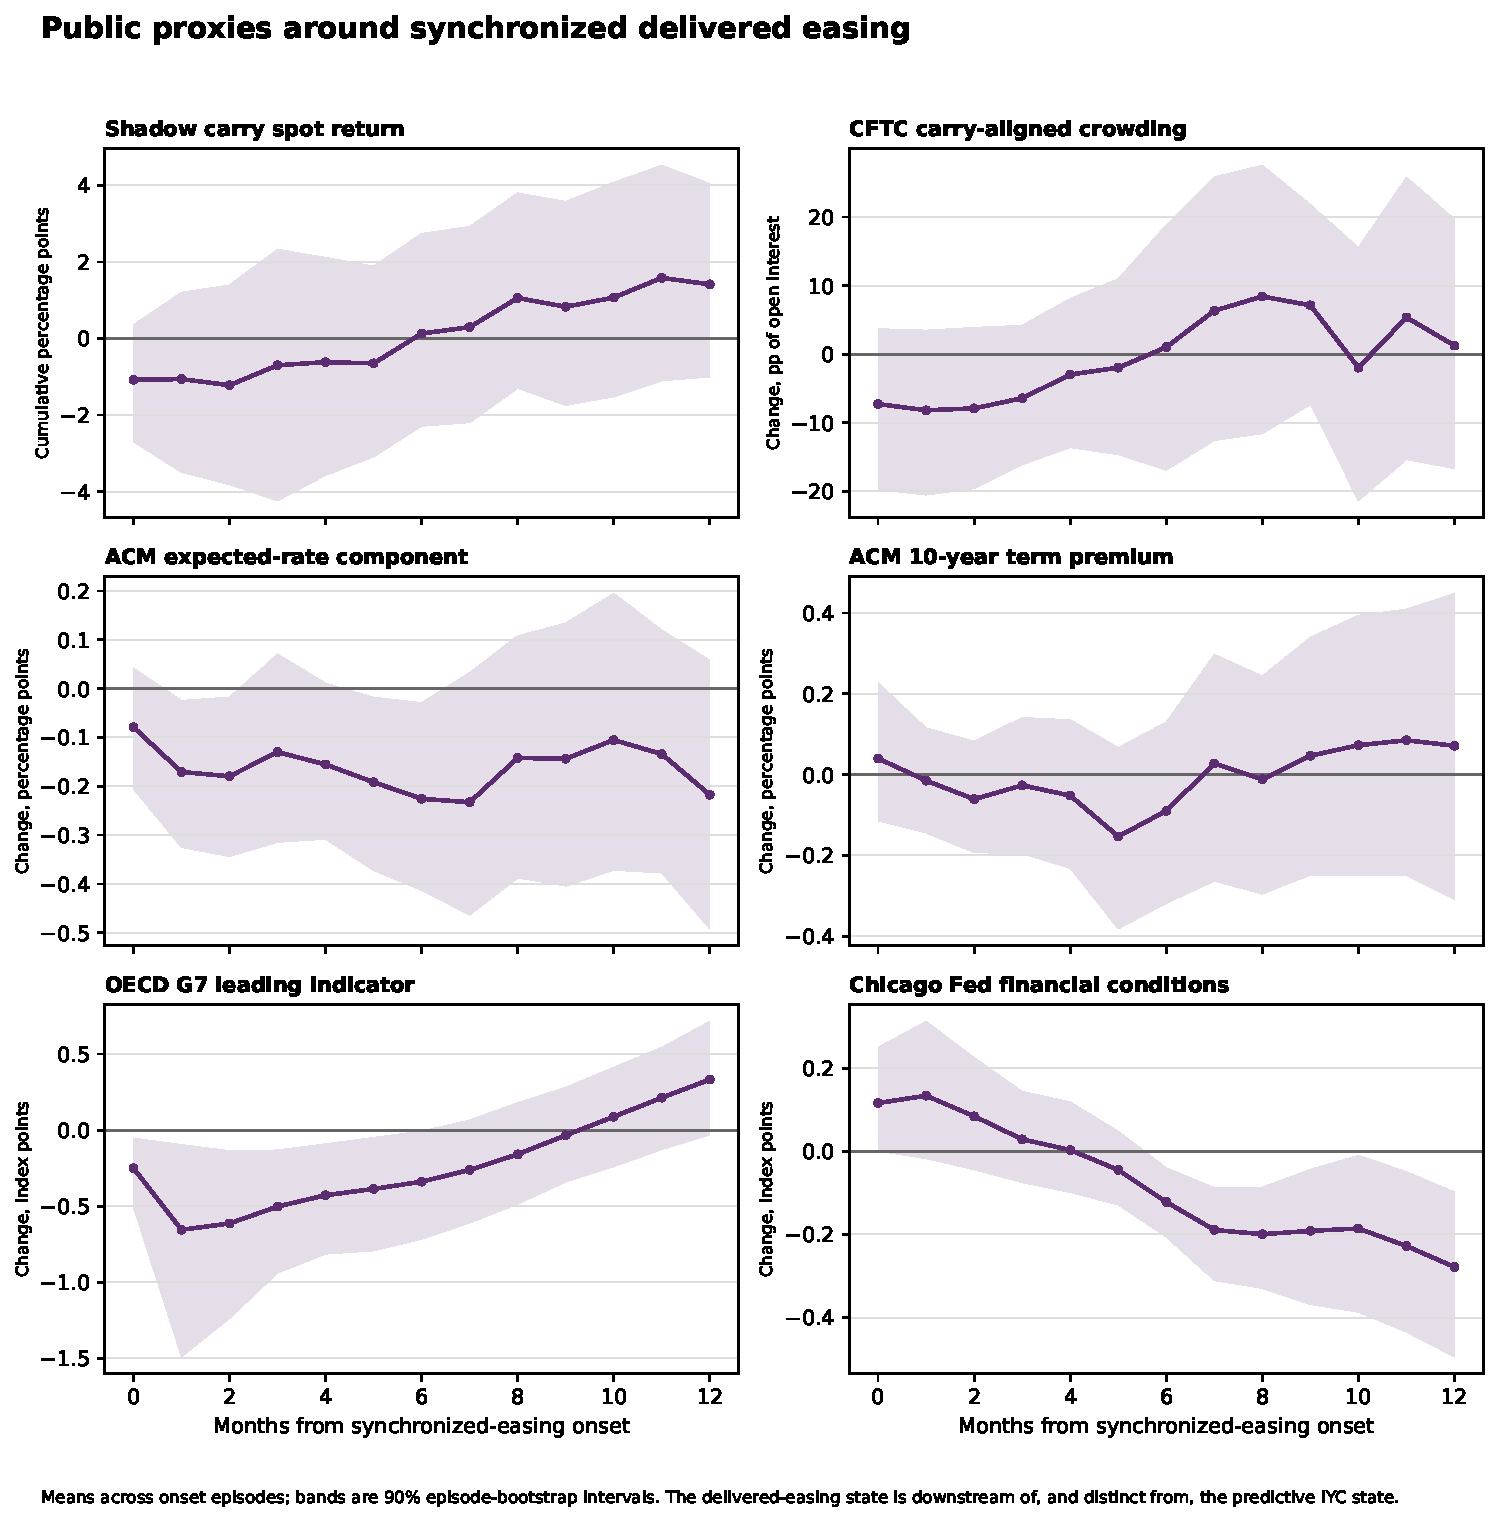
\includegraphics[width=0.86\textwidth]{generated/public_mechanism_event_study.pdf}
  \caption{Outcomes around synchronized delivered-easing onsets. Event time zero is a month in which at least three policy rates fall by at least 10 basis points after a three-month quiet period. Panels show the code-defined cumulative return or endpoint-change estimands, with 90-percent episode-bootstrap intervals.}
  \label{fig:public-event-study}
\end{figure}

\subsection{Sensitivity and interpretation}

The shadow-carry response is recomputed using two- and four-country event thresholds and after omitting each event currency. Every threshold recomputes its own quiet period, so onset counts need not be monotone in the required number of cutting countries.

\begin{table}[H]
\centering
\caption{Public-proxy sensitivity: shadow carry spot return}
\label{tab:public_proxy_sensitivity}
\small
\begin{tabular}{lrrrr}
\toprule
Construction & Estimate & Rotation ref. & Events & Rotations \\
\midrule
At least three countries easing & -1.06 & 0.222 & 15 & 441 \\
At least two countries easing & -1.10 & 0.120 & 22 & 434 \\
At least four countries easing & -0.40 & 0.694 & 18 & 438 \\
Exclude AUD from event rule & -0.56 & 0.515 & 17 & 439 \\
Exclude CAD from event rule & 0.35 & 0.548 & 18 & 438 \\
Exclude CHF from event rule & -1.21 & 0.132 & 15 & 441 \\
Exclude EUR from event rule & -1.02 & 0.182 & 16 & 440 \\
Exclude GBP from event rule & -0.83 & 0.294 & 20 & 436 \\
Exclude JPY from event rule & -0.24 & 0.838 & 19 & 437 \\
Exclude NOK from event rule & -1.53 & 0.072 & 13 & 443 \\
Exclude NZD from event rule & -0.53 & 0.590 & 15 & 441 \\
Exclude SEK from event rule & -0.40 & 0.702 & 17 & 439 \\
\bottomrule
\end{tabular}
\begin{minipage}{0.92\linewidth}\footnotesize Notes: Each threshold definition recomputes its own three-month quiet window. Onset counts therefore need not be monotone in the number of countries required to cut. Leave-one-currency rows omit that currency from the event rule.\end{minipage}
\end{table}


The exercise has four binding limits. Delivered easing is endogenous to prior information and occurs downstream of the paper's predictor. Policy-rate ranks are not money-market or forward rates, and spot returns omit carry income, basis, transaction costs, and implementation lags. CFTC, ACM, and current-vintage macro series are imperfect proxies for the intended objects. Finally, fifteen onsets---fewer for some outcomes---leave low episode-level power. The public results are therefore useful as a reproducible challenge to mechanism implications, not as a replication of the headline state.
